\chapter{長弦與黑洞對應}

\lectureoverview{黑洞具有熵，因此必定擁有微觀自由度。我們將建立最簡單的弦論描述來說明這些自由度：先計數長激發弦的態，再改變弦耦合，直到弦與黑洞的描述相互銜接。最後的等式刻意留作下一講要完成的問題。}

\section{熵意味著存在微觀載體}

說一個系統具有很大的熵，就是說它能隱藏大量微觀資訊。一浴缸熱水的熵可能高達\(10^{30}\)。這已足以告訴我們，系統有極其大量的微觀自由度，無論我們是否逐一檢視其中的分子。熱力學可以透過測量能量和溫度來確定熵，卻無法指出哪些物件承載了這些熵。

流體動力學讓這種區分顯得很熟悉。它描述密度、速度、壓力和宏觀流動，卻不提原子。加入熱力學後，我們便會發現流體具有熵。熵揭示了粗粒化方程中看不見的微觀結構；它引出新的問題，卻不會回答問題。

黑洞以更鮮明的方式提出同樣的挑戰。Bekenstein提出的想法，經由Hawking的計算而確立：熵正比於視界面積。廣義相對論決定了幾何及其熱力學，卻沒有列出微觀態。究竟是哪些微小而眾多的物件，其組態能解釋面積律？弦理論提供了一個具體的候選答案。這裡的論證刻意採取定性方式：它給出正確的參數依賴關係，但省略數值常數，也不採用完整態計數所需的形式化工具。

\section{三個尺度與一個記號陷阱}

引力提供了一個特徵長度，即普朗克長度，
\begin{equation}
\ell_p=\sqrt{\frac{G_N\hbar}{c^3}}.
\label{eq:l06-planck-si}
\end{equation}

\begin{classroomqa}
\audiencequestion{\(G_N\)、\(\hbar\)和\(c\)要如何組合，才能得到普朗克長度？\lecturetimestamp{00:06:08}}
\lecturerresponse{答案是\(\sqrt{G_N\hbar/c^3}\)，約為\(10^{-33}\)公分。我們立刻令\(\hbar=c=1\)，這樣關係式就簡單多了。}
\end{classroomqa}

在自然單位制下，
\begin{equation}
\hbar=c=1,
\qquad
G_N=\ell_p^2.
\label{eq:l06-planck-area}
\end{equation}
因此，牛頓常數的量綱是面積。這就是為什麼面積除以\(G_N\)後是無量綱量，因而可以作為熵。

弦理論還有第二個長度，\(\ell_s\)。加熱一條弦，或使它處於高度激發態，弦便會在許多尺度上振動。在這個簡化圖像中，特徵性的最短尺度就是弦長。可以把\(\ell_s\)看作一個基本弦振動單元所對應的尺度。

第三個量是無量綱的弦耦合\(g_s\)。它控制弦的分裂與合併：一條弦可以分裂成兩條弦，激發弦也可以發射一個閉弦量子。

\begin{classroomqa}
\audiencequestion{弦耦合的物理意義是什麼？\lecturetimestamp{00:09:20}}
\lecturerresponse{它控制弦發生交互作用的機會，例如弦與自身相交時可能分裂。更精確地說，\(g_s\)是交互作用振幅；相應的機率或速率則從\(g_s^2\)階開始。}
\end{classroomqa}

發射出的無質量閉弦激發可以是引力子。在這方面，\(g_s\)的作用類似電荷：它是附在交互作用頂點上的因子。\editorialnote{本講有時把\(g_s\)稱為機率，有時又稱為振幅。在微擾論中，它是振幅層級的耦合；機率和速率則包含它的平方。}

\section{為何引力會受到\texorpdfstring{\(g_s^2\)}{耦合平方的影響}}

先來看電磁學中的交換圖像。一個帶電物體發射光子時會帶有一個\(e\)因子，第二個物體吸收光子時又帶有一個\(e\)因子，因此交換振幅包含\(e^2\)。這不是字面上的經典拋射物圖像，但能正確呈現耦合如何進入。

\begin{figure}[htbp]
\centering
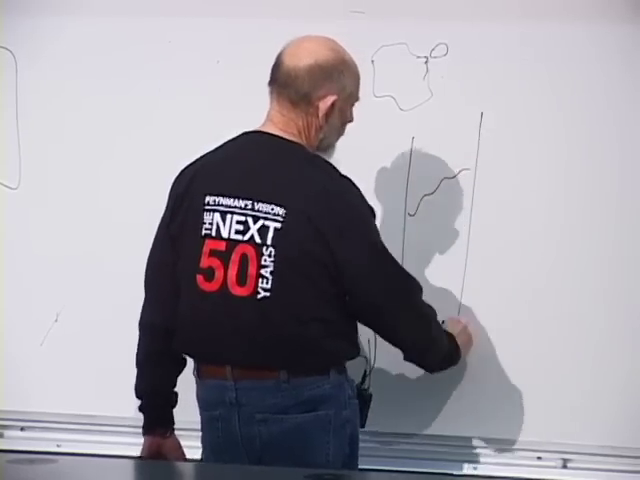
\includegraphics[width=0.72\textwidth]{lecture_06_figure_03.png}
\caption{黑板上完成的交換示意圖：發射處帶有一個耦合因子，吸收處也帶有一個。}
\lectureframe{00:11:30.000}
\end{figure}

在弦理論中，以引力子取代光子，以\(g_s\)取代電荷。發射和吸收各帶有一個因子，因此引力強度正比於\(g_s^2\)。

在長距離下，同一種交互作用必須重現牛頓力定律，
\begin{equation}
F_{\mathrm{grav}}\sim G_N\frac{M_1M_2}{r^2}.
\end{equation}
質量和平方反比關係描述了源與傳播；此處的重點是乘在它們前面的耦合。

\begin{figure}[htbp]
\centering
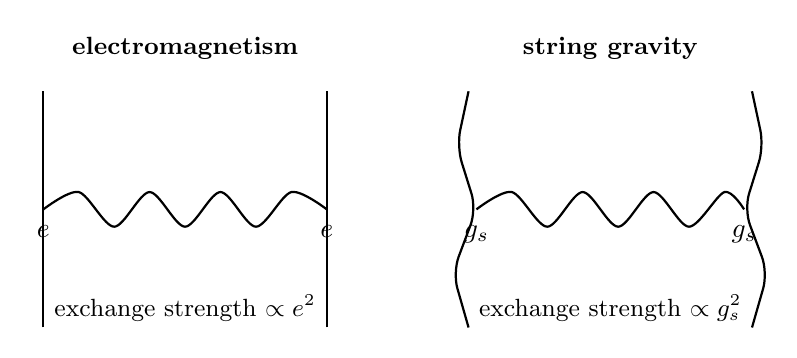
\begin{tikzpicture}[x=1cm,y=1cm]
  \node[font=\small\bfseries] at (1.8,3.55) {electromagnetism};
  \draw[line width=0.8pt] (0,0) -- (0,3);
  \draw[line width=0.8pt] (3.6,0) -- (3.6,3);
  \draw[line width=0.8pt] plot[smooth] coordinates {(0,1.5) (0.45,1.72) (0.9,1.28) (1.35,1.72) (1.8,1.28) (2.25,1.72) (2.7,1.28) (3.15,1.72) (3.6,1.5)};
  \node[below] at (0,1.42) {\(e\)};
  \node[below] at (3.6,1.42) {\(e\)};
  \node[font=\small] at (1.8,0.25) {exchange strength \(\propto e^2\)};
  \node[font=\small\bfseries] at (7.2,3.55) {string gravity};
  \draw[line width=0.8pt,rounded corners=6pt] (5.4,0) -- (5.2,0.7) -- (5.5,1.5) -- (5.25,2.3) -- (5.4,3);
  \draw[line width=0.8pt,rounded corners=6pt] (9,0) -- (9.2,0.7) -- (8.9,1.5) -- (9.15,2.3) -- (9,3);
  \draw[line width=0.8pt] plot[smooth] coordinates {(5.5,1.5) (5.95,1.72) (6.4,1.28) (6.85,1.72) (7.3,1.28) (7.75,1.72) (8.2,1.28) (8.65,1.72) (8.9,1.5)};
  \node[below] at (5.5,1.42) {\(g_s\)};
  \node[below] at (8.9,1.42) {\(g_s\)};
  \node[font=\small] at (7.2,0.25) {exchange strength \(\propto g_s^2\)};
\end{tikzpicture}
\caption{耦合計數的類比：交換量子的兩端各貢獻一個交互作用因子。}
\end{figure}

這個觀察幾乎足以確定牛頓常數。耦合\(g_s\)是無量綱的，而在四維中，\(G_N\)的量綱是長度平方。可用的微觀長度是\(\ell_s\)，因此
\begin{equation}
G_N\sim g_s^2\ell_s^2.
\label{eq:l06-newton-string}
\end{equation}
將此結果與方程~\eqref{eq:l06-planck-area}合併，得到
\begin{equation}
\ell_p\sim g_s\ell_s.
\label{eq:l06-planck-string}
\end{equation}

\begin{figure}[htbp]
\centering
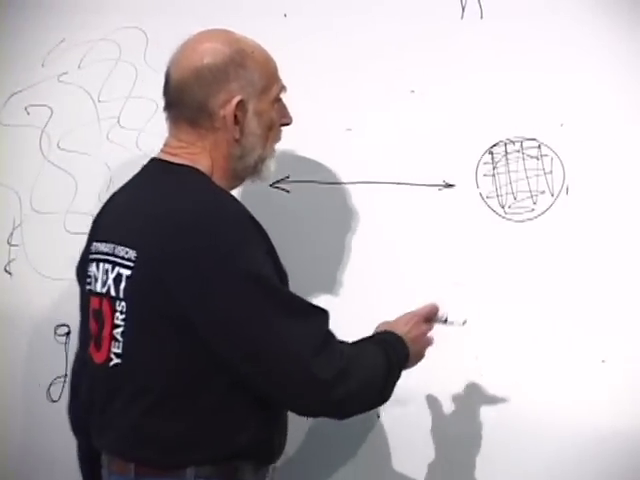
\includegraphics[width=0.72\textwidth]{lecture_06_figure_04.png}
\caption{黑板上保留的基本關係：\(\ell_p^2=G_N\)和\(\ell_p\sim g_s\ell_s\)。}
\lectureframe{00:15:45.000}
\end{figure}

方程~\eqref{eq:l06-newton-string}是本講全程採用的簡化關係。\editorialnote{在緊緻化弦理論中，有效四維牛頓常數也取決於緊緻化體積和一些量級為一的約定。本講省略這些因素，以凸顯對應關係的標度。}

\begin{classroomqa}
\audiencequestion{\(g_s\)是大於還是小於一？哪個長度比較大？\lecturetimestamp{00:16:00}}
\lecturerresponse{我們考慮弱耦合情況，\(g_s<1\)。於是，\(\ell_p\sim g_s\ell_s\)表示弦長大於普朗克長度。強耦合需要另一種描述，此處不必討論。}
\end{classroomqa}

\section{黑洞的熵計數}

略去波茲曼常數和數值因子後，Bekenstein--Hawking熵為
\begin{equation}
S_{\mathrm{BH}}=\frac{A}{4G_N}sim\frac{A}{G_N}sim\frac{A}{\ell_p^2}.
\label{eq:l06-bh-area}
\end{equation}
因子\(1/4\)在半經典公式中是精確的，但對這裡的標度論證沒有影響。

\begin{classroomqa}
\audiencequestion{下標``BH''是指黑洞，還是Bekenstein--Hawking？\lecturetimestamp{00:16:51}}
\lecturerresponse{就本講的目的而言，它可以同時讓我們想到兩者。重要的是，熵等於以普朗克面積為單位計量的視界面積。}
\end{classroomqa}

對於四維Schwarzschild黑洞，
\begin{equation}
R_s=2G_NM,
\qquad
A=4\pi R_s^2.
\end{equation}
如本講所做，略去\(2\)和\(4\pi\)後，
\begin{align}
S_{\mathrm{BH}}
&\sim \frac{R_s^2}{G_N}
\sim \frac{(G_NM)^2}{G_N} \\
&\sim M^2G_N
\sim M^2\ell_p^2.
\label{eq:l06-bh-mass}
\end{align}
這就是接下來要與弦的態計數比較的形式。

\section{長弦如同隨機遊走}

從一條小弦開始，向其中注入能量。一般的高度激發弦不會維持整齊的環狀，而會變成一個長而纏結的物體，就像魚線嚴重打結後的樣子。這種纏結具有熵，因為有大量組態在宏觀上看起來相同。

為了計數這些組態，把空間換成一個點陣，格線長度為\(\ell_s\)。格點是頂點，格線是線段，基本方格是面元。弦以一串相連的格線表示。這個模型刻意做得很粗略，但其態數的指數成長能呈現所需的標度。

\begin{figure}[htbp]
\centering
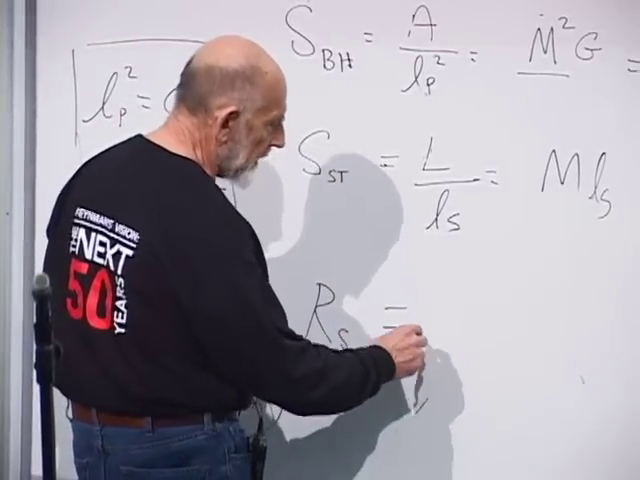
\includegraphics[width=0.72\textwidth]{lecture_06_figure_05.png}
\caption{二維點陣模型。藍色線段表示弦的一步；每到一個格點，就計入四種可能的延伸方向。}
\lectureframe{00:23:50.000}
\end{figure}

\begin{classroomqa}
\audiencequestion{這個簡化的隨機遊走，每一步有幾種選擇？\lecturetimestamp{00:22:43}}
\lecturerresponse{在正方點陣上有四種，因為允許立即折返。在三維則有六種。換用其他點陣會改變這個具體數字，但遊走數目會隨格線數呈指數成長，這點不變。}
\end{classroomqa}

若弦含有\(n\)條格線，二維簡化模型的計數為
\begin{equation}
\Omega_n\sim4^n.
\label{eq:l06-walk-count}
\end{equation}
有一種例外情況是筆直前進的遊走，但在\(4^n\)個態中，它只占一個。典型的遊走會不斷折返，形成一團纏結的球狀物。當\(n\)很大時，幾乎所有隨機生成的組態在定性上都大同小異。

熵是宏觀上無法區分的組態數目之對數：
\begin{equation}
S_{\mathrm{st}}=\log\Omega_n\sim n\log4\sim n.
\label{eq:l06-string-entropy-n}
\end{equation}

\begin{classroomqa}
\audiencequestion{為什麼熵正比於\(n\)，而不是\(4^n\)？\lecturetimestamp{00:25:39}}
\lecturerresponse{熵是態數的對數。因此\(\log(4^n)=n\log4\)，而因子\(\log4\)是量級為一的常數，我們會略去它。}
\end{classroomqa}

如果\(L\)表示沿著弦從一端走到另一端所得的輪廓長度，那麼
\begin{equation}
n=\frac{L}{\ell_s},
\qquad
S_{\mathrm{st}}\sim\frac{L}{\ell_s}.
\label{eq:l06-string-entropy-length}
\end{equation}
此處的\(L\)不是纏結球的直徑，而是沿弦測量、長得多的距離。

接下來，我們把輪廓長度換成質量。在\(c=\hbar=1\)下，質量的量綱是長度的倒數。因此，一條弦尺度的格線所帶的質量約為
\begin{equation}
m_{\mathrm{link}}\sim\frac{1}{\ell_s}.
\label{eq:l06-link-mass}
\end{equation}

\begin{classroomqa}
\audiencequestion{為什麼一條格線的質量必須正比於\(1/\ell_s\)？\lecturetimestamp{00:29:20}}
\lecturerresponse{在這些單位下，質量是長度的倒數，而\(\ell_s\)是唯一可用的長度。等價地說，量級為\(1/\ell_s^2\)的弦張力乘上格線長度\(\ell_s\)，也會得到相同結果。}
\end{classroomqa}

因此，整條弦的量為
\begin{equation}
M\sim n m_{\mathrm{link}}
\sim\frac{n}{\ell_s}
\sim\frac{L}{\ell_s^2},
\qquad
L\sim M\ell_s^2.
\label{eq:l06-string-mass}
\end{equation}
代入方程~\eqref{eq:l06-string-entropy-length}便得到
\begin{equation}
S_{\mathrm{st}}\sim M\ell_s.
\label{eq:l06-string-entropy-mass}
\end{equation}
點陣遊走模型忽略了世界面約束和數值係數，但高度激發弦譜的指數成長仍給出相同的主導標度。\editorialnote{隨機遊走是理解弦態高能階密度的簡便圖像，並非將基本弦真的離散化。}

\section{引出這套論證的不一致}

現在得到的兩個結果是
\begin{equation}
S_{\mathrm{BH}}\sim M^2\ell_p^2,
\qquad
S_{\mathrm{st}}\sim M\ell_s.
\label{eq:l06-two-entropies}
\end{equation}
兩者形式相似，但在固定質量和任意耦合下並不相等。黑洞的熵對\(M\)呈二次關係，弦的熵則呈線性關係。不能只說熱弦就是黑洞，還必須說明兩種情況如何銜接。

\begin{figure}[htbp]
\centering
\includegraphics[width=0.78\textwidth]{lecture_06_figure_06.png}
\caption{黑板上完整呈現的比較：上方是黑洞熵，下方是長弦熵，左側保留普朗克--弦關係。}
\lectureframe{00:33:20.000}
\end{figure}

課堂在此停了下來。這個懸念有其用處：兩者不一致並不代表想法行不通，反而提示我們應在改變引力強度時，追蹤同一個態來進行比較。

\section{轉動耦合旋鈕}

固定\(\ell_s\)，並設想\(g_s\)可以改變。在\(g_s=0\)時，弦既不分裂也不合併；由於\(G_N\sim g_s^2\ell_s^2\)，引力也會消失。此時，能量足夠高的態就是一條長而弱交互作用的弦。

緩慢增大\(g_s\)。弦交互作用因此成為可能；而對這裡的論證來說，更重要的是引力增強了。

\begin{classroomqa}
\audiencequestion{隨著\(g_s\)增大，最先發生的是否只是弦分裂成較短的弦？\lecturetimestamp{00:36:29}}
\lecturerresponse{弦的分裂與合併會變得可能，但要固定\(\ell_s\)並追蹤這個高熵態。關鍵效應是\(G_N\)增大，使長弦的自引力將纏結成團的弦往內拉。}
\end{classroomqa}

物體會收縮並變得更緻密。它的引力位能為負，因此收縮會降低總能量，也就降低了質量。

\begin{classroomqa}
\audiencequestion{自引力把弦拉攏時，能量會增加還是減少？\lecturetimestamp{00:37:48}}
\lecturerresponse{會減少，因為束縛能變得更負。雖然我們持續追蹤同一個態，沿途的質量卻不一定保持不變。}
\end{classroomqa}

最後，物體的尺度會接近其Schwarzschild半徑。到達這一點後，用黑洞來描述便最為自然。初始激發越大，達到這個條件所需的耦合越小，因為質量越大的物體形成視界所需的引力越弱。

\begin{figure}[htbp]
\centering
\resizebox{0.95\linewidth}{!}{%
\begin{tikzpicture}[x=1cm,y=1cm,>=Latex]
  \draw[->,line width=0.9pt] (0,0) -- (11,0) node[right] {increasing \(g_s\)};
  \node[draw,rounded corners,align=center,minimum width=2.6cm,minimum height=1.15cm] at (1.8,1.5) {long excited string\\weak self-gravity};
  \node[draw,rounded corners,align=center,minimum width=2.6cm,minimum height=1.15cm] at (5.5,1.5) {correspondence point\\\(R_s\sim\ell_s\)};
  \node[draw,circle,align=center,minimum size=1.8cm] at (9.3,1.5) {black\\hole};
  \draw[->,line width=0.8pt] (3.15,1.5) -- (4.1,1.5) node[midway,above,font=\small] {contracts};
  \draw[->,line width=0.8pt] (6.9,1.5) -- (8.25,1.5);
  \node[font=\small,align=center] at (5.5,-0.65) {same family of states followed slowly;\\binding energy and mass may change};
\end{tikzpicture}
}
\caption{固定\(\ell_s\)時的對應路徑。反轉箭頭，就會把黑洞態轉變回長弦態。}
\end{figure}

\begin{classroomqa}
\audiencequestion{我們是否應設想\(g_s\)介於零與一之間？\lecturetimestamp{00:40:18}}
\lecturerresponse{是的。這套論證仍處於弱耦合範圍。如果\(g_s\)非常小，該態就必須具有相應大的質量才會成為黑洞。我們不必進入難以控制的\(g_s>1\)範圍。}
\end{classroomqa}

在這個思想實驗中，緩慢變化是可逆的。

\begin{classroomqa}
\audiencequestion{如果把耦合調低，直到引力無法再束縛黑洞，它會變成什麼？\lecturetimestamp{00:41:37}}
\lecturerresponse{一條長弦。當引力消失時，這套構造中的一切都必須以弦態描述。朝一個方向轉動旋鈕，會使弦態轉變為黑洞態；反向轉動，則會使黑洞態轉變為弦態。}
\end{classroomqa}

在總能量和體積固定時，主導的高熵組態基本上是一條長弦，而不是數量極多的短弦。這裡不推導這個結論；它是弦在Hagedorn區域附近的統計力學結果，之後會再討論。

\section{外部觀察者看到什麼}

當物體被描述為黑洞時，弦在哪裡？在外部觀察者的描述中，弦不會突然消失。以Schwarzschild時間來看，弦穿越視界的表象會延至任意晚的時刻，因此弦的自由度會被描述為在視界上或附近累積。

\begin{figure}[htbp]
\centering
\includegraphics[width=0.72\textwidth]{lecture_06_figure_07.png}
\caption{黑板上的比較：對宏觀視界而言，弦尺度的結構只像一層薄霧；較小的視界半徑則逐漸接近環的尺度。}
\lectureframe{00:45:30.000}
\end{figure}

當\(R_s\gg\ell_s\)時，黑洞是宏觀的，弦尺度的結構相較於視界半徑只是一層薄薄的區域。半徑縮小至接近\(\ell_s\)時，平滑黑洞與延展弦之間的區別便失去意義。這是外部觀察者採用的拉伸視界描述；不應把它誤解為一項與座標無關的主張，認為落入的物質永遠不會穿過正常的視界。\editorialnote{本講採用的是黑洞互補性中熟悉的外部描述。短語``在視界上''指的是外部描述所能分辨的自由度，並非對其協變位置另行推導的結果。}

交叉發生在
\begin{equation}
R_s\sim\ell_s.
\label{eq:l06-correspondence-radius}
\end{equation}
低於弦尺度時，Schwarzschild幾何無法分辨原本應支撐它的結構。弦環會從可能的視界位置向外漲落，此時稱該態為弦更為恰當。

\section{對應點}

將\(R_s\sim G_NM\)代入方程~\eqref{eq:l06-correspondence-radius}：
\begin{equation}
G_NM\sim\ell_s.
\end{equation}
接著代入\(G_N\sim g_s^2\ell_s^2\)：
\begin{equation}
M g_s^2\ell_s^2\sim\ell_s,
\qquad
M g_s^2\ell_s\sim1.
\label{eq:l06-correspondence-condition}
\end{equation}

\begin{figure}[htbp]
\centering
\includegraphics[width=0.72\textwidth]{lecture_06_figure_08.png}
\caption{黑板上完成的轉換運算：由\(R_s\sim\ell_s\)可得加框的無量綱條件\(Mg_s^2\ell_s\sim1\)。}
\lectureframe{00:49:50.000}
\end{figure}

一位聽眾注意到這個條件正是為了導出什麼。在對應點，
\begin{align}
S_{\mathrm{BH}}
&\sim M^2\ell_p^2
\sim M^2g_s^2\ell_s^2 \\
&=(M\ell_s)(Mg_s^2\ell_s)
\sim M\ell_s
\sim S_{\mathrm{st}}.
\label{eq:l06-entropy-preview}
\end{align}

\begin{classroomqa}
\audiencequestion{這些方程是否已經表示黑洞熵和弦熵相等？\lecturetimestamp{00:50:18}}
\lecturerresponse{是的，計算正是要導出這個結果。各項要素都已列在黑板上，但本講暫緩完整推導，以便仔細回顧對應關係的邏輯。}
\end{classroomqa}

方程~\eqref{eq:l06-entropy-preview}是這段問答中隱含的一行代數預覽。它確立的是標度關係，而非精確係數\(1/4\)。要精確匹配微觀態，需要採用控制得更好的黑洞和更詳細的弦理論構造。\editorialnote{本講在呈現方程~\eqref{eq:l06-entropy-preview}的完整推導之前便告一段落。由於聽眾明確指出這個等式，而且所需的關係式都已出現，這裡便將等式寫出。}

\section{熵為何能沿途保持不變}

還有一個邏輯環節。假設系統保持孤立且演化可逆，並且緩慢改變某個控制參數，例如磁場或\(g_s\)。能量、大小和束縛能都可能改變，但熵保持不變：
\begin{equation}
\Delta S=0.
\label{eq:l06-adiabatic-entropy}
\end{equation}
本講將此與資訊守恆相連。熵衡量粗粒化描述所隱藏的資訊；緩慢且可逆地改變哈密頓量，只會重新排列各態，不會刪除這些資訊。

\begin{classroomqa}
\audiencequestion{熵保持不變是否要求路徑避開相變？\lecturetimestamp{00:54:01}}
\lecturerresponse{是的，必須能夠連續追蹤該態。有限系統不會發生無限體積系統那種嚴格非解析的熱力學相變；若變化足夠緩慢，便可將對應視為平滑的交叉。}
\end{classroomqa}

此處所說的絕熱，採用的是較嚴格的準靜態、可逆意義。絕熱但不可逆的過程仍可能產生熵；因此，緩慢變化以及能夠追蹤該態都不可或缺。\editorialnote{熱力學陳述\(\Delta S=0\)要求路徑可逆且絕熱。在量子力學中，對應的想法是隨著參數改變，持續追蹤同一組態，不發生無法控制的能階躍遷。}

\begin{classroomqa}
\audiencequestion{為什麼一條長弦的熵會高於攜帶相同總質量的幾條短弦？\lecturetimestamp{00:54:44}}
\lecturerresponse{這確實違反直覺，但對高能態進行明確計數後可知，在固定體積中，含有長弦成分的組態較受偏好。證明暫且留待後續；目前的論證只需要知道，黑洞會對應到熵最大的弦態區域，而非由大量短弦組成的稀薄氣體。}
\end{classroomqa}

因此，具體做法如下：
\begin{enumerate}
\item 從耦合為\(g_{s,0}\)、質量為\(M_0\)的黑洞開始。
\item 緩慢降低\(g_s\)，同時追蹤同一族高熵態。
\item 在\(R_s\sim\ell_s\)時停止；此時黑洞描述轉變為長弦描述。
\item 利用\(S_{\mathrm{st}}\sim M\ell_s\)計算弦態數目。
\item 沿可逆路徑把此熵帶回原來的黑洞。
\end{enumerate}

\begin{figure}[htbp]
\centering
\includegraphics[width=0.72\textwidth]{lecture_06_figure_09.png}
\caption{陳述策略時，黑板上保留的原則是：絕熱改變\(g_s\)不會改變\(S\)。}
\lectureframe{00:56:40.000}
\end{figure}

弦理論已經為帶電、旋轉、超對稱、近極端及高維黑洞提供更精確的熵計數。此處討論的中性Schwarzschild黑洞，只涉及粗略的對應論證：它找出態密度的參數依賴關係和物理上的交叉點，而非精確且受保護的簡併度。\editorialnote{對於耦合改變時態計數仍受保護的特殊黑洞，兩種描述的一致性最為有力。本講刻意只介紹最簡單的量級估算。}

\begin{classroomqa}
\audiencequestion{引力關閉後，這個態會不會變成兩條弦，而非恰好一條？\lecturetimestamp{00:58:25}}
\lecturerresponse{出現少數幾條長弦的機率不為零；用兩條弦而非一條弦，不會改變熵的主導標度。會改變論證的是弦碎裂成由大量短弦組成的氣體；高能統計計數並不支持這種情況。}
\end{classroomqa}

黑洞是在一個區域內能夠容納的最大熵；移除引力後，相應的高熵態則是長弦。兩種描述如今已經連結起來，但還沒有發展成精確計算。接下來要仔細重做代數推導，並探討這種對應關係究竟能在多大範圍內成立。
